% Brief Process Step
\chapter{Process Step}
\section{TFT Dimension}
\label{thickness}
\subsection{Film Thickness}
\begin{enumerate}
\item Source-Drain electrode, Aluminum: 60 (desired) -- 70 nm.
\item n+ nc-Si:H contact layer: 60 (desired) -- 70 nm.
\item a-Si:H channel layer: 60 (desired) -- 70 nm.
\item a-SiN\subscript{x}:H gate dielectric: 300 nm.
\item Gate electrode, Aluminum: 100 nm. (Figure only has up to this level)
\item a-SiN\subscript{x}:H Insulation layer: 300 nm.
\item Top electrode, Aluminum: 1000 nm. (Not shown in the figure below)
\end{enumerate}
\begin{figure}[ht]
  \centering
  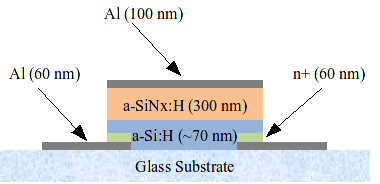
\includegraphics[width=0.7\textwidth]{TFT_Dimension.png}
  \caption{A TFT schematic of current process.}
  \label{fig:TFT_side}
\end{figure}
\subsection{Film Recipe}
\begin{enumerate}
\item Aluminum: WLOS.
\item a-Si:H: (Kodak PL2) Originally developed for Kodak project. Table \ref{tab:a-SiKai}
\item n+ nc-Si:H: Mohammad, newest one. (So far, best dark conductivity from WLO1)
\item a-SiN\subscript{x}:H: Hadi. (Requires film test at this moment)
\end{enumerate}

\section{Fabrication Procedure}
\begin{figure}[ht]
  \centering
  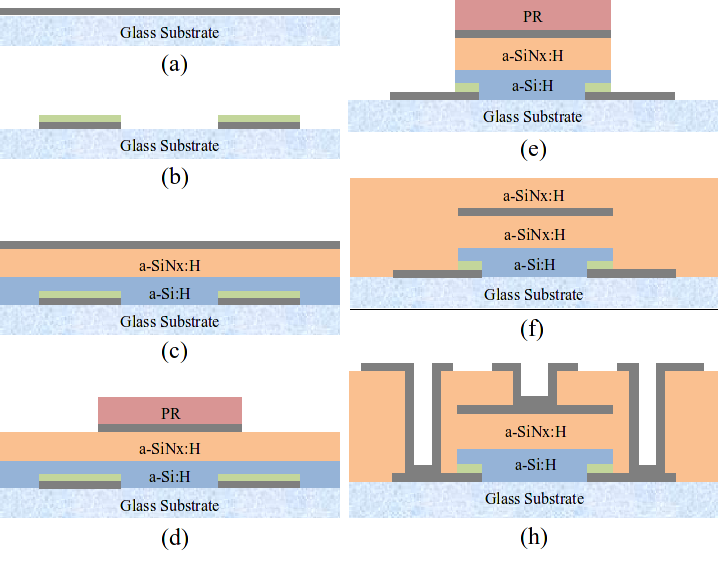
\includegraphics[width=0.8\textwidth]{ProcessFlow.png}
  \caption{Fabrication procedure.}
  \label{fig:TFT_Process}
\end{figure}
The process is consisted of four lithography steps as illustrated in Figure \ref{fig:TFT_Process}.  The etching time of each films and surface profile should be monitored throughout the process.
\begin{enumerate}
\item Mask \#1 (L1) \\
  After lithography, n+ nc-Si:H will be etched by RIE while source-drain electrodes will be etched by PAN. The etch speed for n+ film is quite fast, 30 sec is good enough for 60 -- 70 nm n+ while the Al is opposite case; 5 mins for 60 nm. Lastly, A few seconds of \textbf{BHF(or 2\% HF if exercise extreme care) dip} will be required before a-Si:H and a-SiN\subscript{x}:H deposition to remove naturally grown Silicon Dioxide(SiO\subscript{2}) on n+ nc-Si:H film.
\item Mask \#2 (L2) \\
  The 100 nm top electrode shall be deposited right after gate dielectric(a-SiN\subscript{x}) deposition. The patterning will define gate electrode, therefore, with 25 $\mu$m gap between gate and source-drain electrodes will be observable. The gate dielectric and channel layers will be etched by Hyun-Jung's RIE recipe shown in Tab. \ref{tab:RIE-HJLEE}, resulting Fig. \ref{fig:TFT_Process} (e). The discrete devices are ready to test once PR stripped from gate electrode. Using molybdenum causes overetch problem in RIE process losing the Source-Drain electrodes due to strong RIE plasma. Moreover, Hadi's a-SiN\subscript{x} recipe is not recommended for such thick application(300 nm in this case) due to PR lift-off problem.
\item Mask \#3 (L4) \\
  For VCO patterns, we need to deposit additional a-SiN\subscript{x}:H film to passivate TFTs since an additional path required. The passivation a-SiN\subscript{x}:H will be patterned by RIE, using negative mask, Mask \#3.
\item Mask \#4 (L3) \\
  The additional path for VCO is implemented here. Since we need wirebonding for VCO patterns, the electrode, must be 'Aluminum' having thickness at least 800 nm. (300 nm if you are able to use mechanical engineering facility) Therefore, Edwards will be used.
\item Lastly, but optionally, we can anneal the devices under 250 \superscript{o}C about 3 hours to improve device characteristics. 
\end{enumerate}
